
\documentclass[border=10pt, 12pt]{standalone}
\usepackage[svgnames]{xcolor}
\usepackage{amsmath}
\usepackage{pgfplots}
\pgfplotsset{compat=newest}
\usepackage[sfdefault]{FiraSans}
\usepackage{FiraMono}
\renewcommand*\familydefault{\sfdefault}
\begin{document}
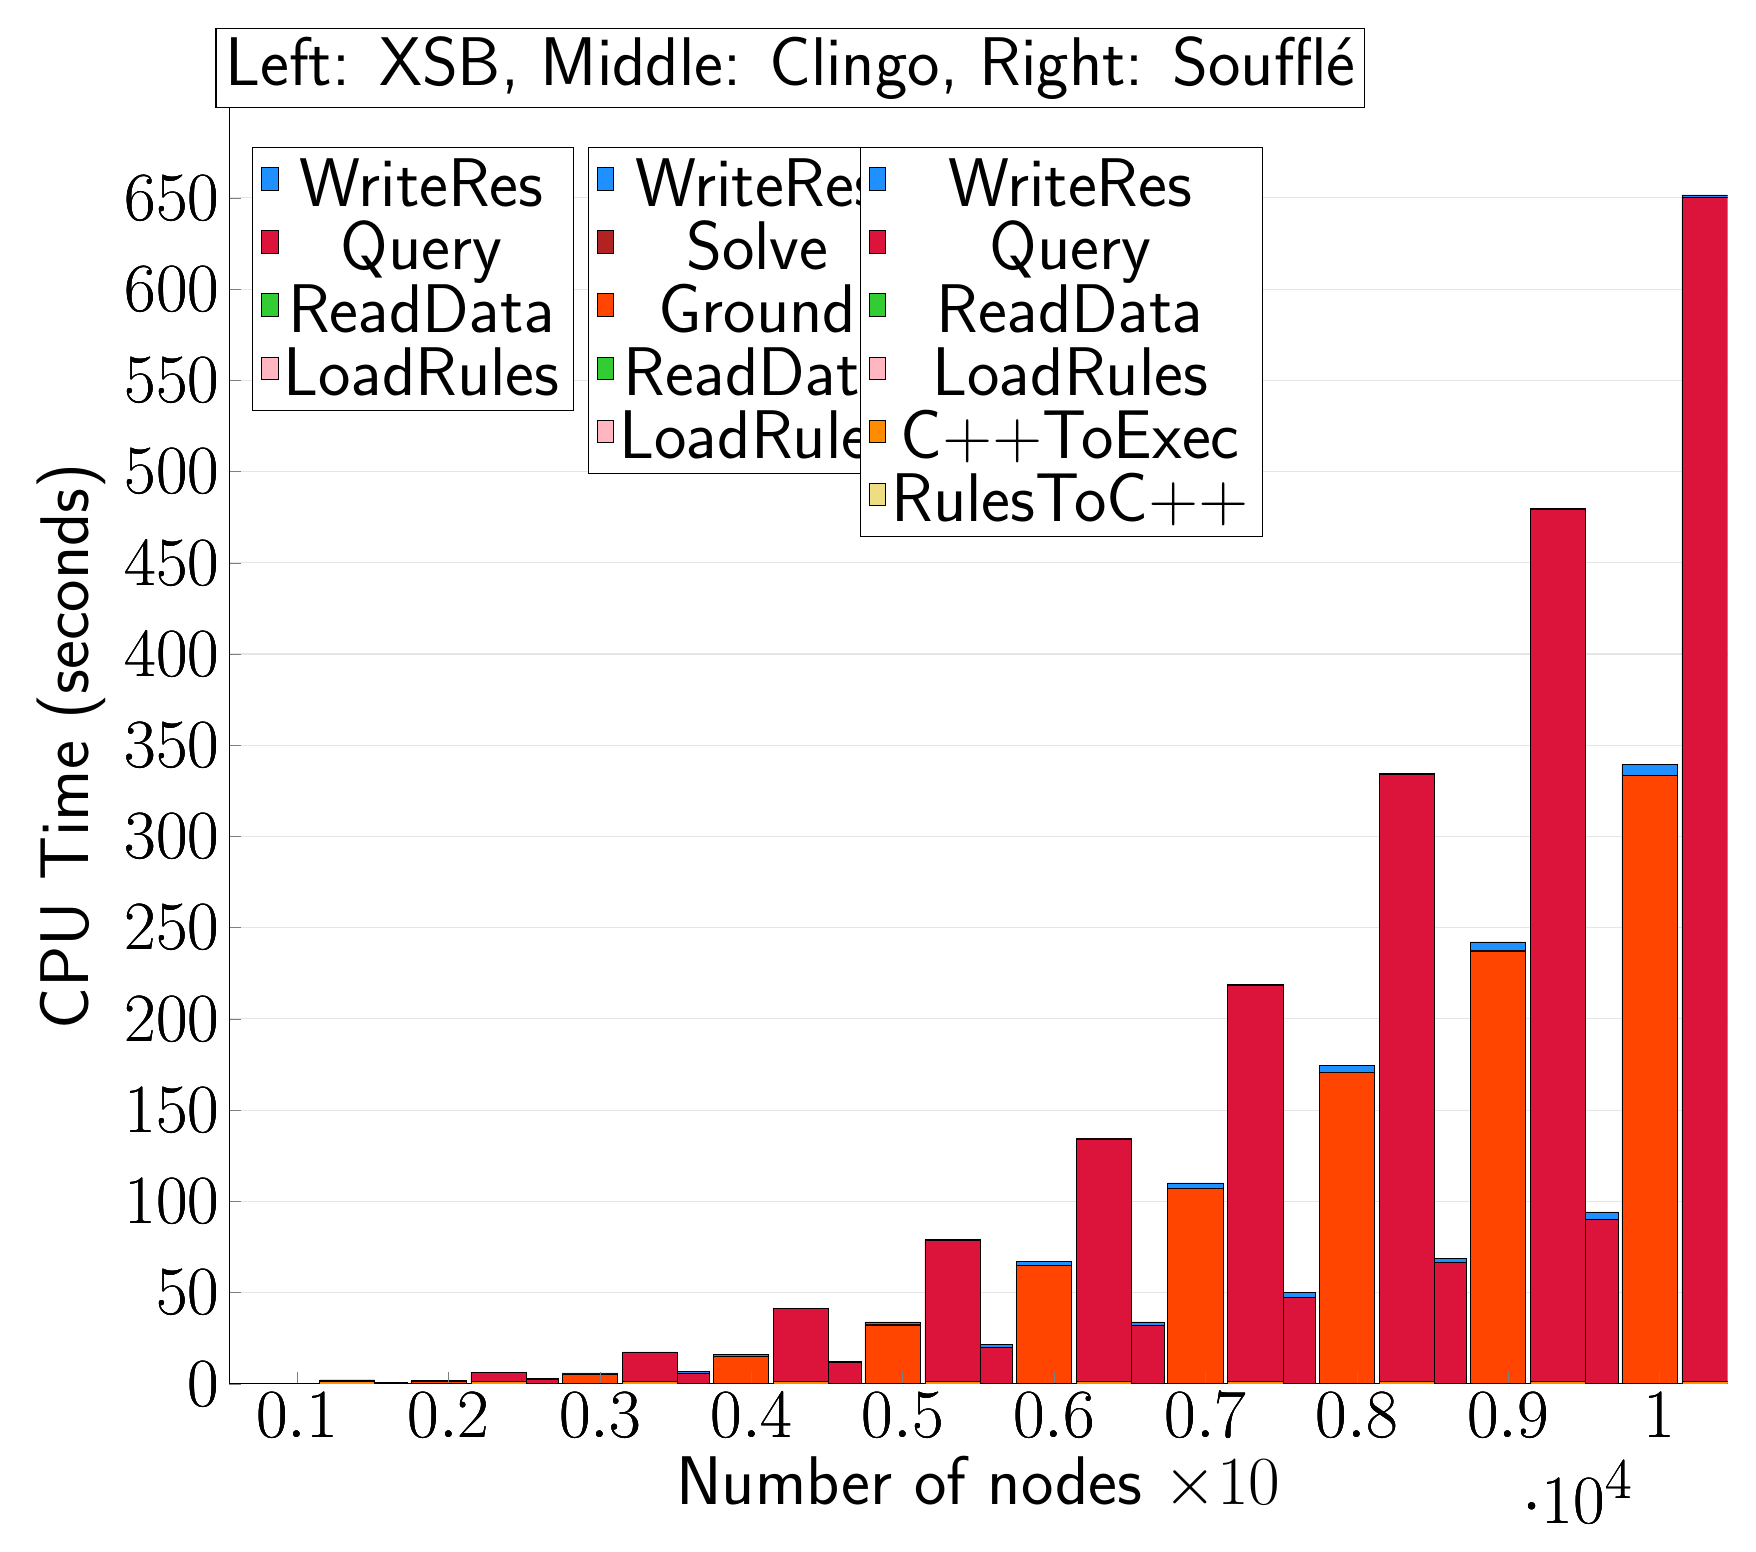
\begin{tikzpicture}
                        \begin{axis}[bar shift=-25pt, 
   ybar stacked,
   width=1.7\textwidth,
   bar width=0.7cm,
   ymajorgrids, tick align=inside,
   major grid style={draw=gray!20},
   xtick=data,
   ymin=0, ymax=699.059,
   axis x line*=bottom,
   axis y line*=left,
   enlarge x limits=0.05,
   legend style={
       at={(0.23, 0.97)},
       anchor=north east,
       legend columns=1,
       font=\Huge,
   },
   ylabel={CPU Time (seconds)},
   xlabel={Number of nodes $\times 10$},
   label style={font=\Huge},
   tick label style={font=\Huge},
]
\addlegendimage{fill=DodgerBlue, draw=black, line width=0.2pt}
\addlegendentry{WriteRes}
\addlegendimage{fill=Crimson, draw=black, line width=0.2pt}
\addlegendentry{Query}
\addlegendimage{fill=LimeGreen, draw=black, line width=0.2pt}
\addlegendentry{ReadData}
\addlegendimage{fill=LightPink, draw=black, line width=0.2pt}
\addlegendentry{LoadRules}
\addplot +[fill=LightPink, draw=black, line width=0.2pt] coordinates {
(1000, 0.0005490000000000002)
(2000, 0.0005472000000000003)
(3000, 0.0005485999999999995)
(4000, 0.0005480000000000001)
(5000, 0.0005476000000000011)
(6000, 0.0005464)
(7000, 0.0005506000000000004)
(8000, 0.000549)
(9000, 0.0005514000000000003)
(10000, 0.0005478000000000003)
};
\addplot +[fill=LimeGreen, draw=black, line width=0.2pt] coordinates {
(1000, 0.0008948000000000001)
(2000, 0.0017182)
(3000, 0.0025402000000000003)
(4000, 0.00337)
(5000, 0.0041928)
(6000, 0.0050304)
(7000, 0.0058444)
(8000, 0.0066968)
(9000, 0.007470599999999999)
(10000, 0.008323)
};
\addplot +[fill=Crimson, draw=black, line width=0.2pt] coordinates {
(1000, 0.097403)
(2000, 0.7729158)
(3000, 2.5408991999999997)
(4000, 6.0029965999999995)
(5000, 11.542550199999999)
(6000, 20.159913)
(7000, 32.062797)
(8000, 47.2948454)
(9000, 66.60956580000001)
(10000, 89.93197340000002)
};
\addplot +[fill=DodgerBlue, draw=black, line width=0.2pt] coordinates {
(1000, 0.041442200000000005)
(2000, 0.1576306)
(3000, 0.36377999999999994)
(4000, 0.7362394)
(5000, 0.9154564000000004)
(6000, 1.3768538)
(7000, 1.887247)
(8000, 2.607070399999999)
(9000, 2.0817780000000026)
(10000, 4.305703799999998)
};
\end{axis}

\begin{axis}[bar shift=-3.7pt, 
   ybar stacked,
   width=1.7\textwidth,
   bar width=0.7cm,
   ymajorgrids, tick align=inside,
   major grid style={draw=none},
   xtick=data,
   ymin=0, ymax=699.059,
   axis x line*=none,
   axis y line*=none,
   enlarge x limits=0.05,
   legend style={
       at={(0.454, 0.97)},
       anchor=north east,
       legend columns=1,
       font=\Huge,
   },
   label style={font=\Huge},
   tick label style={font=\Huge},
]
\addlegendimage{fill=DodgerBlue, draw=black, line width=0.2pt}
\addlegendentry{WriteRes}
\addlegendimage{fill=FireBrick, draw=black, line width=0.2pt}
\addlegendentry{Solve}
\addlegendimage{fill=OrangeRed, draw=black, line width=0.2pt}
\addlegendentry{Ground}
\addlegendimage{fill=LimeGreen, draw=black, line width=0.2pt}
\addlegendentry{ReadData}
\addlegendimage{fill=LightPink, draw=black, line width=0.2pt}
\addlegendentry{LoadRules}
\addplot +[fill=LightPink, draw=black, line width=0.2pt] coordinates {
(1000, 0.0)
(2000, 0.0)
(3000, 0.0)
(4000, 0.0)
(5000, 0.0)
(6000, 0.0)
(7000, 0.0)
(8000, 0.0)
(9000, 0.0)
(10000, 0.0)
};
\addplot +[fill=LimeGreen, draw=black, line width=0.2pt] coordinates {
(1000, 0.0)
(2000, 0.0)
(3000, 0.0)
(4000, 0.008000000000000007)
(5000, 0.010000000000000009)
(6000, 0.010000000000000009)
(7000, 0.014000000000000012)
(8000, 0.010000000000000009)
(9000, 0.020000000000000018)
(10000, 0.022000000000000013)
};
\addplot +[fill=OrangeRed, draw=black, line width=0.2pt] coordinates {
(1000, 0.192)
(2000, 1.4680000000000002)
(3000, 5.401999999999999)
(4000, 14.942000000000002)
(5000, 32.348)
(6000, 64.96199999999999)
(7000, 107.07199999999997)
(8000, 170.502)
(9000, 237.31)
(10000, 333.25199999999995)
};
\addplot +[fill=FireBrick, draw=black, line width=0.2pt] coordinates {
(1000, 0.0020000000000000018)
(2000, 0.014000000000000012)
(3000, 0.024000000000000025)
(4000, 0.04799999999999969)
(5000, 0.0779999999999987)
(6000, 0.11600000000000228)
(7000, 0.16)
(8000, 0.2080000000000036)
(9000, 0.264)
(10000, 0.3519999999999841)
};
\addplot +[fill=DodgerBlue, draw=black, line width=0.2pt] coordinates {
(1000, 0.057999999999999996)
(2000, 0.22799999999999992)
(3000, 0.5319999999999998)
(4000, 0.9319999999999998)
(5000, 1.4480000000000028)
(6000, 2.0579999999999963)
(7000, 2.8379999999999996)
(8000, 3.6640000000000015)
(9000, 4.6119999999999965)
(10000, 5.748000000000035)
};
\end{axis}

\begin{axis}[bar shift=18pt, 
   ybar stacked,
   width=1.7\textwidth,
   bar width=0.7cm,
   ymajorgrids, tick align=inside,
   major grid style={draw=none},
   xtick=data,
   ymin=0, ymax=699.059,
   axis x line*=none,
   axis y line*=none,
   enlarge x limits=0.05,
   legend style={
       at={(0.69, 0.97)},
       anchor=north east,
       legend columns=1,
       font=\Huge,
   },
   label style={font=\Huge},
   tick label style={font=\Huge},
]
\addlegendimage{fill=DodgerBlue, draw=black, line width=0.2pt}
\addlegendentry{WriteRes}
\addlegendimage{fill=Crimson, draw=black, line width=0.2pt}
\addlegendentry{Query}
\addlegendimage{fill=LimeGreen, draw=black, line width=0.2pt}
\addlegendentry{ReadData}
\addlegendimage{fill=LightPink, draw=black, line width=0.2pt}
\addlegendentry{LoadRules}
\addlegendimage{fill=DarkOrange, draw=black, line width=0.2pt}
\addlegendentry{C++ToExec}
\addlegendimage{fill=LightGoldenrod, draw=black, line width=0.2pt}
\addlegendentry{RulesToC++}
\addplot +[fill=LightGoldenrod, draw=black, line width=0.2pt] coordinates {
(1000, 0.004000000000000001)
(2000, 0.0020000000000000005)
(3000, 0.004000000000000001)
(4000, 0.0)
(5000, 0.0020000000000000005)
(6000, 0.0)
(7000, 0.0020000000000000005)
(8000, 0.007999999999999997)
(9000, 0.0)
(10000, 0.003999999999999997)
};
\addplot +[fill=DarkOrange, draw=black, line width=0.2pt] coordinates {
(1000, 1.4740000000000002)
(2000, 1.474)
(3000, 1.47)
(4000, 1.468)
(5000, 1.472)
(6000, 1.4779999999999998)
(7000, 1.48)
(8000, 1.476)
(9000, 1.482)
(10000, 1.4760000000000002)
};
\addplot +[fill=LightPink, draw=black, line width=0.2pt] coordinates {
(1000, 0.00018119999999999999)
(2000, 0.0001794)
(3000, 0.000196)
(4000, 0.0002058)
(5000, 0.0002204)
(6000, 0.00020119999999999998)
(7000, 0.00018020000000000002)
(8000, 0.00019260000000000002)
(9000, 0.0001938)
(10000, 0.0002056)
};
\addplot +[fill=LimeGreen, draw=black, line width=0.2pt] coordinates {
(1000, 0.004066600000000001)
(2000, 0.007144599999999999)
(3000, 0.0102306)
(4000, 0.0137874)
(5000, 0.0153112)
(6000, 0.018166)
(7000, 0.0180116)
(8000, 0.020606400000000004)
(9000, 0.022085800000000003)
(10000, 0.025811999999999995)
};
\addplot +[fill=Crimson, draw=black, line width=0.2pt] coordinates {
(1000, 0.6201072)
(2000, 4.8246780000000005)
(3000, 15.861160000000002)
(4000, 39.852419999999995)
(5000, 77.29784)
(6000, 132.69580000000002)
(7000, 216.7926)
(8000, 332.5596)
(9000, 477.6094)
(10000, 649.059)
};
\addplot +[fill=DodgerBlue, draw=black, line width=0.2pt] coordinates {
(1000, 0.0108664)
(2000, 0.0432386)
(3000, 0.09741740000000002)
(4000, 0.17434319999999998)
(5000, 0.2687214)
(6000, 0.384685)
(7000, 0.526432)
(8000, 0.6820733999999999)
(9000, 0.8626343999999999)
(10000, 1.065892)
};
\end{axis}


\node[anchor=south, draw, fill=white] at (rel axis cs:0.42,1) {\Huge Left: XSB, Middle: Clingo, Right: Soufflé};
\end{tikzpicture}
\end{document}
                    